To meet the requirements and goals of the project it was clear that a platform was needed that could compile and run code. An initial suggestion from the project description was to use \techio{}, which is a collaborative platform to share coding assignments through open-source ``playgrounds''. The platform seemed to match the needs of the project and the project owner had been in touch with the developers, but no API access had been guaranteed.
\begin{figure}[ht]
    \begin{subfigure}{.45\linewidth}
        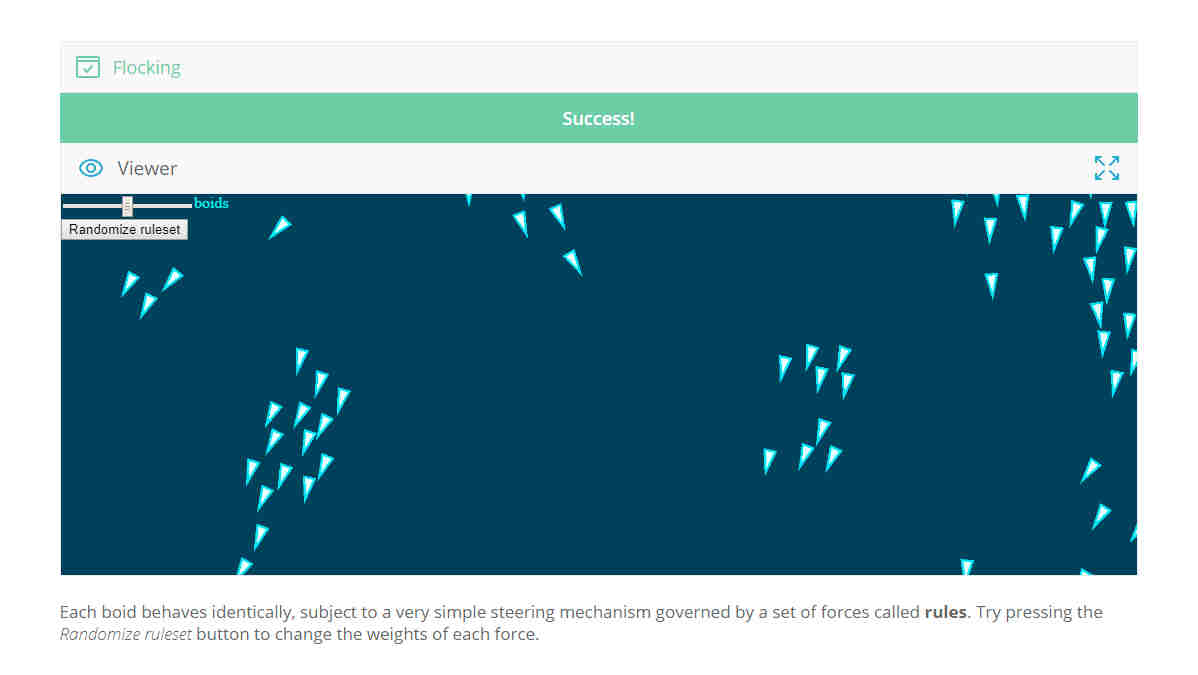
\includegraphics[width=\linewidth]{img/techio_game.jpg}
        \caption{One of the games.}
    \end{subfigure}
    \hfill
    \begin{subfigure}{.45\linewidth}
        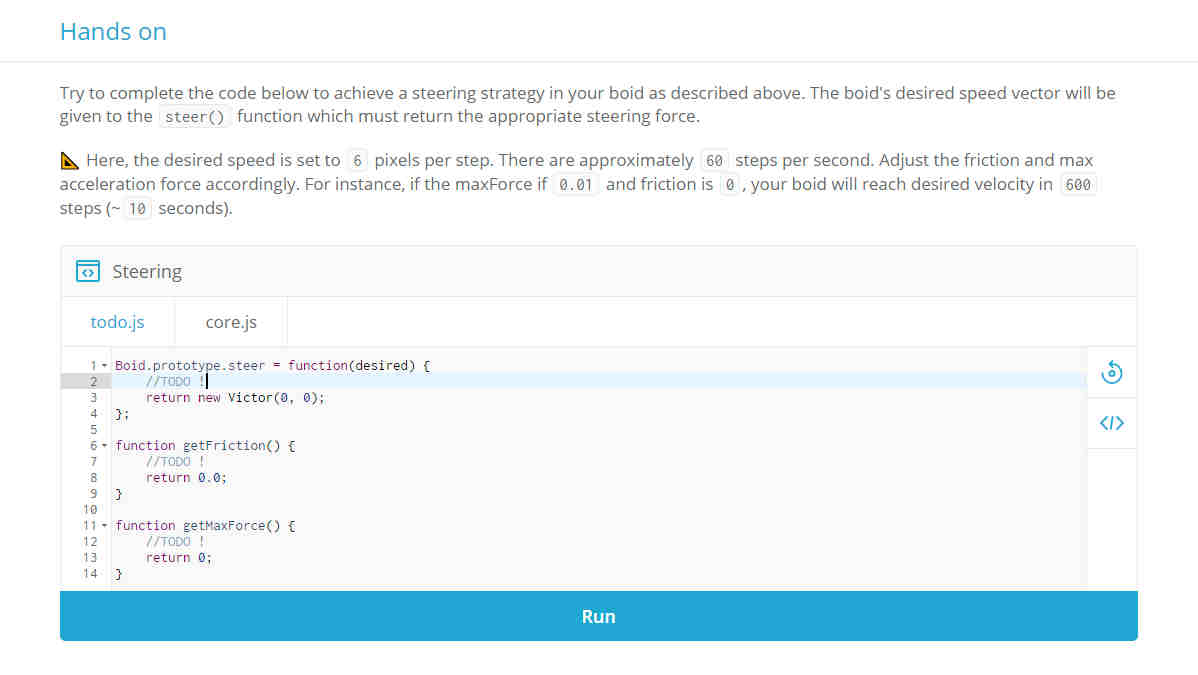
\includegraphics[width=\linewidth]{img/techio_handson.jpg}
        \caption{Coding in \techio.}
    \end{subfigure}
    \caption{Example pictures from \techio.}
\end{figure}

After some investigation into the platform and discussion with the developers, it was found that \techio{} does not have---and will not get---any open APIs. Thus, the only possibility of using their system was to  embed ``code snippets'' from their site into the one that was to be built. Because of this shortcoming, \techio{} was discarded.

In contrast to \techio{}, a student at \LTU{} has developed an open platform called \sockr{} for hosting programming ladders. However, while the solution was more interesting from the licensing point of view, \sockr{} didn't have any documentation and required too much refactoring to be of use for the project.
